\documentclass[a4paper,11pt]{scrartcl}

\usepackage{graphicx}
\usepackage[utf8]{inputenc}
\usepackage{amsmath,amssymb,amsthm} 
%\usepackage[round]{natbib}
\usepackage{url}
\usepackage{xspace}
\usepackage[left=20mm,top=20mm]{geometry}
\usepackage{algorithmic}
\usepackage{subcaption}
\usepackage{mathpazo}
\usepackage{booktabs}
\usepackage{hyperref}
\usepackage{tikz}

\usetikzlibrary{matrix, shapes, arrows, positioning, chains}
% \usepackage{draftwatermark}

\newcommand{\ie}{ie}
\newcommand{\eg}{eg}
\newcommand{\reffig}[1]{Figure~\ref{#1}}
\newcommand{\refsec}[1]{Section~\ref{#1}}

\setcapindent{1em} %-- for captions of Figures

\renewcommand{\algorithmicrequire}{\textbf{Input:}}
\renewcommand{\algorithmicensure}{\textbf{Output:}}

% Define block styles
\tikzset{
    decision/.style={
        diamond,
        draw,
        text width=4em,
        text badly centered,
        inner sep=0pt
    },
    block/.style={
        rectangle,
        draw,
        text width=10em,
        text centered,
        rounded corners
    },
    cloud/.style={
        draw,
        ellipse,
        minimum height=2em
    },
    descr/.style={
        fill=white,
        inner sep=2.5pt
    },
    connector/.style={
        -latex,
        font=\scriptsize
    },
    rectangle connector/.style={
        connector,
        to path={(\tikztostart) -- ++(#1,0pt) \tikztonodes |- (\tikztotarget) },
        pos=0.5
    },
    rectangle connector/.default=-2cm,
    straight connector/.style={
        connector,
        to path=--(\tikztotarget) \tikztonodes
    }
}



\title{cgFRAMES}
\author{Lennart de Bruin}
\date{\today}


\begin{document}

\maketitle

\tableofcontents

\section{Introduction}

cgFRAMES is a program that fits user-specified atom groups to atom groups in Molecular Dynamics trajectories, and PDB files (not supported yet).

It is set up as follows: the user specifies an ideal atom group in a specified format in a file. This atom group will contain the atom names, and coordinates. On top of that, a frame is specified w.r.t. the origin of the coordinate system the atom coordinates are in.

The program will then find these atoms in the MD topology file, and the corresponding coordinates in the MD trajectory file, fit the ideal atom group to this group in a later specified method, and output the frames for all specified atom groups for each MD snapshot in the .fra format.

\section{Usage}

\subsection{Input files}

\begin{description}
    \item[.top] The topology file. The standard AMBER format.
    \item[.nc] The trajectory file. The standard nc format.
    \item[ideal bases] The file containing the ideal bases. The format is as follows:\\
        Each entry has:\\
        \verb+<group name> <# atoms in group> <9 values of the frame orientation matrix> <3 values of the frame position vector>+\verb\\
        \verb+<x> <y> <z> <atom name as in the topology file> (for each atom)+\verb\\

        Comments begin with an \#. Between each entry there needs to be an empty line, or a comment.
\end{description}

\subsection{Output files}

\section{External libraries}

The program uses netCDF to read in the MD trajectories from Amber MD simulations.

\section{Compilation}

\section{Folder hierarchy}

The hierarchy of the folders is as follows:
\begin{description}
    \item[bin] \hfill \\ contains the binary produced by compiling the program. 
    \item[doc] \hfill \\ contains this document, and other documentation.
    \item[include] \hfill \\ contains all header files
    \item[input] \hfill \\ contains all files necessary for using cgFRAMES. Think of ideal bases.
    \item[output] \hfill \\ contains all files outputted by cgFRAMES.
    \item[src] \hfill \\ contains the implementation files of the program.
    \item[test\_files] \hfill \\ contains main files for testing the implementation. This was originally for unit testing, but the author was too lazy to bother.
    \item[utilities] \hfill \\ contains several scripts to convert the simulations output to different formats, e.g. for viewing the configuration with cgDNAjs.
\end{description}

\section{Program structure}
The structure of the program is laid out in the flow-chart below.

\begin{figure}
    \centering
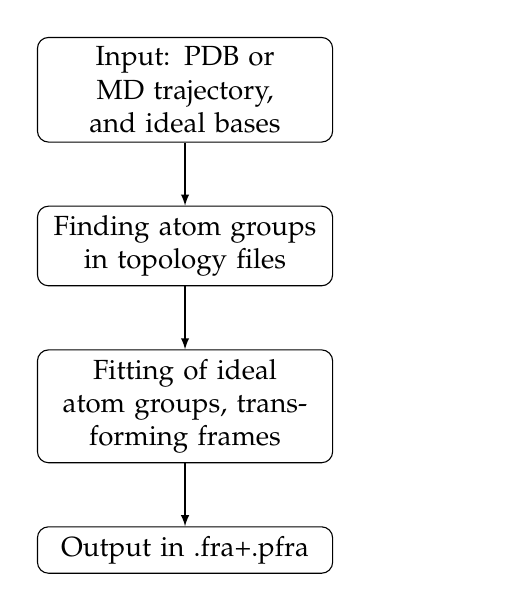
\begin{tikzpicture}
\matrix (m)[matrix of nodes, column  sep=2cm,row  sep=8mm, align=center, nodes={rectangle,draw, anchor=center} ]{
    |[block]| {Input: PDB or MD trajectory, and ideal bases} &  \\
    |[block]| {Finding atom groups in topology files}  & \\
    |[block]| {Fitting of ideal atom groups, transforming frames}  & \\
    |[block]| {Output in .fra+.pfra} &\\
};
\path [>=latex,->] (m-1-1) edge (m-2-1);
\path [>=latex,->] (m-2-1) edge (m-3-1);
\path [>=latex,->] (m-3-1) edge (m-4-1);

\end{tikzpicture}
\end{figure}


\section{Things left to do}
There are a lot of things left to do:
\begin{enumerate}
    \item Finish the PDB format reader, so that frames can also be fitted to PDB files.
    \item At the moment only DNA bases are supported. This needs to be extended to perhaps basepairs, and general atom groups, so that also frames can be fitted to proteins. For this, the topology file needs to be stored in a better way. (At the moment only the atoms are stored, with positions, not the connections between atoms. We can only find DNA bases because the program assumes that the atoms of the bases are next to eachother in the MD topology file).
\end{enumerate}

Where to start:

1. One could download a library to parse the PDB files, since these files tend to vary in which record different information is stored. Libraries that come to mind are one from stanford: \url{http://graphics.stanford.edu/~drussel/pdb}, or the official PDBx/mmCIF reader: \url{http://mmcif.wwpdb.org/docs/sw-examples/cpp/html/index.html}. Then put this in the general protein data structures used by cgFRAMES. 

2. Not only the atoms are specified in the topology files, but also the connections between them. These can be somehow used to see the atoms' relation to the specified groups. This is in general not an easy problem to solve, and impossible if you have disjoint subgroups belonging to the same specified group that are not unique in the set of atoms you're searching in.
%\bibliographystyle{plainnat}
%\bibliography{/Users/hugo/references/references}

\end{document}
